\documentclass[journal,a4paper,twoside]{sty/IEEEtran}

%% Based on bare_jrnl.tex V1.3 2007/01/11 by Michael Shell (requires IEEEtran.cls version 1.7 or later) 

\usepackage[utf8]{inputenc}
\usepackage[slovene]{babel}
\usepackage{sty/EVrevija}

% *** GRAPHICS RELATED PACKAGES ***
\usepackage[pdftex]{graphicx}
\graphicspath{ {./Pictures/} }

% Include all other packages here
\usepackage{textcomp} % need for \textmu
\usepackage{setspace}
\usepackage{color}
\definecolor{light-gray}{gray}{0.95}
\usepackage{listings} % za vključevanje kode
%\usepackage{hyperref}
%\usepackage{amsmath}
%\usepackage{amsthm}
%\usepackage{amssymb}

% correct bad hyphenation here
%\hyphenation{op-tical net-works semi-conduc-tor}

\lstset{
basicstyle=\linespread{0.92}\small,
basewidth={0.5em, 0.3em}
}

\begin{document}

% naslov prispevka, lahko uporabite en linebreak \\
\title{Analiza porazdeljenega programskega jezika Julia in primerjava z dobro znanimi alternativami}

\authors{Jan Pelicon, Blaž Rojc}
\address{Univerza v Ljubljani, Fakulteta za računalništvo in informatiko, Večna pot 113, 1000 Ljubljana, Slovenija}

\abstract{Primerjala sva jezika C/C++ in Python z alternativno izbiro - jezikom Julia.
Ugotovila sva, da se po hitrosti bliža C-ju, prinaša pa fleksibilnost in prijaznost Pythona.
Težava je le v relativni novosti jezika, kar se kaže kot nedokončanost določenih delov.}

\keywords{primerjava programskih jezikov, porazdeljeni programski jeziki, hitrost izvajanja, prijaznost do uporabnika}

%\received{19. oktober, 2010} % datum sprejema članka, lahko pustite prazno
%\review{4. februar, 2011}    % datum odobritve članka, pustite prazno

% Priimki avtorjev in kratek naslov članka za tekočo glavo
\markboth{Pelicon, Rojc}{Analiza in primerjava jezika Julia}

% make the title area
\maketitle

\IEEEpeerreviewmaketitle

% Naslov in kratek povzetek v angleščini
% \english{Analisys and comparison of the Julia programming language}
% {TODO}

\section{Uvod}

Porazdeljeno programiranje predstavlja težavo, s katero se večina programerjev nerada spoprijema.
V čist, striktno determinističen tok programiranja vnaša nepredvidljivost, simultane dogodke, neurejenost in kup varnostnih ter pravilnostnih lukenj.
K zahtevnosti programiranja pa pripomore tudi slaba podprtost porazdeljenega programiranja v bolj permisivnih programskih jezikih - tako Python kot
	JavaScript zahtevata daljšo poglobitev v njune sisteme, ki omogočajo distribucijo problemov po več jedrih ali procesorjih, poleg tega pa zaradi
	svojih omejitev ne morata omogočiti tako nizkonivojnega nadzora in optimizacije kot C.

Tu vstopi Julia, dinamičen, prevajan jezik, prvotno namenjen potrebam numerične analize in računske znanosti, a primeren za obilico problemov, kjer je
	hitrost izvajanja tako pomemben faktor kot enostavnost programiranja.\cite{julia-site}
Obljublja enostavno in učinkovito distribucijo dela, hkrati pa ohranja prijaznost do uporabnika.

\section{Jezik}

Julia predstavlja zanimivo sredino med hitrostjo jezika C in prijaznostjo do uporabnika raznih dinamičnih programskih jezikov, kot so Python, JavaSript,
	MATLAB, Lua, ...

Julia se pred izvajanjem optimizira in prevede v strojno kodo z uporabo programske opreme LLVM\footnote{http://llvm.org/}.
To omogoča učinkovito izrabo pomnilnika in procesorskega časa, posledično pa tvorbo programov, ki se v hitrosti približajo ekvivalentni implementaciji v
	jeziku C.\cite{julia-benchmarks}

Je dinamičen programski jezik v polnem pomenu besedne zveze.
Med drugim omogoča dinamično izpeljavo podatkovnih tipov, modificiranje in izvajanje kode iz besedilnih nizov,\cite{julia-metaprogramming} refleksijo,
	makre in večmetodnost funkcij.

V času, ko sva pisala dokument, je jezik že dosegel različico 1.0, a kljub temu še ni popolnoma stabilen.
Kot je opisano pozneje v poročilu, ostaja še velik del obljubljene funkcionalnosti neimplementirane, medtem ko ima stabilnost in hitrost obstoječe kode
	višjo prioriteto.

\section{Sintaksa}

Razvijalci Julie prihajajo s področja računske teorije in matematike\cite{julia-reasons}.
Želeli so ohraniti MATLAB-ovo prijaznost do uporabnika glede vnašanja matematičnih funkcij, hkrati pa vpeljati splošnost jezika Python.

Primer funkcije v jeziku Julia:
\begin{lstlisting}
function onePassSwaps!(src::AbstractArray{T,1}
                           where T<:Number,
                       pivot::Number)
    
    srcSize = size(src)[1]
    i = 0
    j = srcSize + 1
    
    while i < j
    
        i += 1
        while i <= srcSize && src[i] < pivot
            i += 1
        end
        
        j -= 1
        while j > 0 && src[j] > pivot
            j -= 1
        end
        
        if i >= j
            return (j, srcSize - j)
        end
        
        src[i], src[j] = src[j], src[i]
        
    end
end
\end{lstlisting}

Funkcija je deklarirana kot $function \langle ime\rangle (\langle parametri\rangle )$.
Ime v tem primeru vsebuje klicaj.
Ta po dogovoru označuje, da funkcija spreminja argumente (sicer pa ni potreben).
Parametrom so določeni tipi, kar ni nujno, ampak omogoča prevajalniku, da izvede dodatne optimizacije, ki na parametrih splošnega tipa niso možne.
Določeni tipi so generični, njihovi parametri se nahajajo v zavitih oklepajih.

Deklaraciji sledi telo funkcije, ki se konča z rezervirano besedo $end$.
Ukazi skoraj enaki kot v jeziku MATLAB, le da se v Juliji indeksira z oglatimi oklepaji, okrogli oklepaji kot pripona so rezervirani za klice funkcij.
Poleg tega se indeksi v Juliji tako kot v MATLAB-u začnejo z 1.

Podpičja na koncu ukazov niso nujna.
V jeziku MATLAB se uporabljajo za preprečevanje izpisovanja rezultatov ukazov, v Juliji pa se rezultati ukazov v funkcijah ne izpisujejo, zato so
	za ta namen nepotrebna.

Bloki ukazov se v v jeziku C označujejo z zavitimi oklepaji, v Pythonu pa z zamikom v desno.
Julia za ta namen uporablja rezervirani besedi $begin$ in $end$.
Beseda $begin$ ni vedno nujna, na primer pri stavkih $if$, $for$ in $while$ je dovolj le $end$ na koncu bloka.

Funkcija lahko podobno kot v jeziku Python vrača različne tipe vrednosti glede na dane parametre.
V zgornjem primeru vrne par dveh vrednosti, določen z okroglimi oklepaji.

Ista funkcija v jeziku Python:
\begin{lstlisting}
def onePassSwaps (src: np.ndarray, pivot):

    i = -1
    j = src.size

    while i < j:

        i += 1
        while i < src.size and src[i] < pivot:
            i += 1

        j -= 1
        while j >= 0 and src[j] > pivot:
            j -= 1

        if i >= j:
            return (i, src.size - i)

        src[i], src[j] = src[j], src[i]
\end{lstlisting}

Razlike so minimalne, le indeksi, bloki in deklaracija funkcije so različni.

Ista funkcija v jeziku C:
\begin{lstlisting}
void onePassSwaps(int id) {

    int left_border = starts[id];
    int right_border = ends[id];

    int left_index = left_border - 1;
    int right_index = right_border + 1;

    while (left_index <= right_index) {

        left_index++;
        while (table[left_index] <= pivot[id] &&
               left_index <= right_border)
            left_index++;

        right_index--;
        while (table[right_index] > pivot[id] &&
               right_index >= left_border)
            right_index--;

        if (left_index < right_index) {
            long long mem = table[left_index];
            table[left_index] =
                table[right_index];
            table[right_index] = mem;
        }
    }
    split[id] = right_index + 1;
}
\end{lstlisting}

C obravnava tabele popolnoma drugače način kot Python in Julia, kar se odraža na zelo različen izgled kode.
V tem primeru se podatki nahajajo v globalnih tabelah $starts$, $ends$, $table$, \ldots

Vsaka deklaracija spremenljivke vključuje njen tip, vsak ukaz se zaključi s podpičjem.
Pogoji v stavkih $for$, $if$ in $while$ morajo biti zaprti v okroglih oklepajih.
Vsak blok je zaprt v zavitih oklepajih.

\section{Porazdeljeno računanje}

Julia podpira več oblik delitve dela.
Osredotočila sva se na metode podobne tistim, ki smo jih obravnavali pri predmetu Porazdeljeni sistemi: eksplicitna delitev dela med procesorska jedra in
	pošiljanje dela koprocesorjem - GPE.

Julia v teoriji podpira delitev dela med procesorska jedra na več načinov.
Ti so razdeljeni v dve skupini, na osnovi niti in na osnovi procesov.

\subsection{Večnitenje}

Večnitenje je v Juliji eksperimentalna funkcija.

Uporabnost je bila v času pisanja zelo omejena, saj sta bila na voljo le makra \texttt{@threads}, ki na več nitih paralelno izvede \texttt{for} zanko, in
	\texttt{@threadcall}, ki funkcijo v jeziku C pokliče v ločeni niti.\cite{julia-multithreading}
Druga možnost zahteva pisanje dela programa v drugem programskem jeziku, vendar sva se ji izognila.
Prva pa omogoča določeno stopnjo paralelizacije, kljub temu da morda ni tako učinkovita kot v drugih programskih jezikih.

Število niti, s katerimi naj Julia razpolaga, določimo s sistemsko spremenljivko \texttt{JULIA\_NUM\_THREADS}.
Problem, ki ga želimo paralelizirati, predstavimo kot \texttt{for} zanko, ki iterira in razdeli delo, ki ga želimo reševati vzporedno.
Nad to zanko kličemo makro \texttt{@threads}, ki jo porazdeli med razpoložljive niti.

Ta sistem ni primeren za kompleksnejše probleme, ki zahtevajo sinhronizacijo med nitmi.
Če je to potrebno, je bolje problem razdeliti na več podproblemov in vsakega reševati v ločeni paralelizirani \texttt{for} zanki.
Zaradi eksperimentalnega stanja niti je podpora pri razhroščevanju pomanjkljiva ali celo neobstoječa.\cite{julia-thread-problems}

\subsection{Večprocesnost}

Večprocesnost je veliko bolj fleksibilna možnost.
Procesi se v Juliji lahko dodajajo poljubno med izvajanjem, komunikacija pa poteka prek klicev iz glavnega procesa v ostale.
Največja ovira tega pristopa pa je potreba po eksplicitnem podajanju podatkov med procesi, ki poleg dodane kompleksnosti prinaša še dodatno zahtevnost
	izvajanja in počasnejše računanje.

\section{Primerjava z jezikom Python}

Med dinamičnimi programskimi jeziki po popularnosti trenutno kraljuje Python.\cite{python-tiobe}\cite{python-pypl}
Je anekdotno eden najlažjih jezikov za popolne začetnike, omogoča pa tudi reševanje kompleksnejših problemov s širokim naborom javno dostopnih knjižnic -
	modulov.\cite{python-pypi}

Njegova največja hiba je relativna počasnost.
Python je interpretiran jezik, ki se najprej prevede v bitno kodo, nato pa izvaja v virtualnem stroju.
Posledično se kompleksni programi izvajajo veliko počasneje kot v jeziku C.

Julia ohranja večino prednosti Pythona, predvsem dinamičnost in prijaznost do programerja, prinese pa prednost hitrega izvajanja neposredno prevedene
	kode.

Na žalost Julia ne uživa take stopnje podpore kot Python glede obstoječih knjižnic, kar pa je posledica relativne novosti jezika in pomanjkanja izkušenih,
	zavzetih programerjev.
K večji sprejetosti jezika naj bi v prihodnosti pripomogla tudi večja zanesljivost, ki naj bi prišla z uporabo jezika v večjih projektih.

\subsection{Python multiprocessing}

Za deljenje dela med jedra sta na voljo v Pythonu modula “multiprocessing”\footnote{https://docs.python.org/3.7/library/multiprocessing.html} in
	“threading”\footnote{https://docs.python.org/3.7/library/threading.html}, a na žalost se zaradi globalnega zaklepanja interpreterja
	(GIL)\cite{python-gil} v CPython implementaciji lahko izvaja naenkrat le koda ene niti v vsakem Python procesu.
Za učinkovito deljenje dela moramo torej uporabiti modul “multiprocessing”.
Ta nam omogoča zaganjanje poljubnega števila procesov in deljenje podatkov med njimi.

Tako kot v drugih programskih jezikih je tudi v Pythonu delo s procesi precej počasnejše kot z nitmi, ampak dokler je globalni zaklep prisoten, nimamo
	možnosti izbire.

\section{Primerjava z jezikom C/C++}

C je učinkovit nizkonivojski programski jezik, katerega zansova leži zelo blizu strojne kode. 
Njegov naslednik C++, ki se je razvil kot njegova razširitev, ohranja hitrost in prednost, da se prevede v strojni jezik, kar omogoča, da program izvaja
	bistveno hitreje od ostalih programskih jezikov.
Prav tako dopušča precej svobode pri ravnanju s pomnilnikom pri čemer lahko dober programer to izkoristi v svoj prid.
Slabost tega je, da moramo biti zelo pazljivi pri pisanju, če se hočemu izogniti mučnemu in dolgotrajnemu razhroščevanju. 

Omeniti moramo tudi vrsto različnih knjižnic in API-jev, ki uporabniku olajšajo delo in široko podporo, ki jo uživa C++.
Vendar kljub vsem prednostim, pa delo z njim včasih težavno, saj moramo večino dela postoriti sami, medtem ko so višjenivojske funkcije in udobnost
	programiranja stalnica pri nekaterih drugih jezikih. 

\subsection{pthreads}

Pri C++ imamo velik izbor knjižnic za paralelno procesiranje in nitenje.
Nekatere omogočaje več svobode pri upravljanju z njimi, druge pa delitev dela poenostavijo in optimizirajo. 

POSIX Threads ali krajše pthreads so nizkonivojski API za delo z nitmi.
Dopušča nam veliko nadzora in modularnosti za ceno nekoliko kompleksnejše implementacije.
Pazljivi moramo biti predvsem z konfliktnimi dostopi in sinhronizacijo.
Uporabniku omogoča nadzor nad nitjo (kreiranje, uničevanje, odklapljanje,...), upravljanje ključavnic, sinhronizacijo niti z uporabo zapornic in pogojne
	spremenljivke.

\subsection{OpenMP}

Višjenivosjki OpenMP (Open Multi-Processing) predstavlja nekoliko drugačen način razporejanja dela.

Je zbirka direktiv prevajalniku in je nekoliko lažje nastavljiv, sintaktično krajši ter bolj enostaven v primerjavi s pthreads.
Uporabja posebne oznake (\#pragma), ki služijo kot navodila prevajalniku in zagotavlja široko izbiro visoko in nižjenivojskih opcij.
Pomembna lastnost pragme je tudi da v kolikor jo prevajalnik ne prepozna, preprosto nadaljuje z izvajanjem programa. Ta možnost 
omogoča programerju lažje razhroščevanje kot tudi enostavno določanje kaj se bo izvajalo paralelno. 

Njegova hitrost v nekaterih primerih prekaša hitrost pthreads ali pa je približno enaka. Poleg preprostosti ponuja zelo zanesljivo in hitro vzporedno procesiranje.

\section{Algoritma}
Za primerjavo jezikov sva implementirala dva algoritma.

Prvi, Adaptive Quick Sort, je paralelna implementacija sortirnega algoritma Quick Sort.
Izvajal se je na vseh razpoložljivih nitih sistema.
Zasnovala sva ga tako, da vzporedno izvede čim večji del računanja, tudi deljenje in združevanje podatkov.

Z drugim algoritmom pa sva simulirala JPEG kompresijo.
Izvajal se je na grafični kartici prek knjižnic OpenCL in CUDAnative.

\subsection{Adaptive Quick Sort}

Veliko vzporednih implementacij algoritma Quick Sort paralelizira le sortiranje, ne pa tudi deljenja in združevanja podatkov.
Adaptive Quick Sort porazdeli vse, kar omogoča hitrejše izvajanje pri zelo velikih naborih podatkov.

Idejno se vsak korak algoritma izvede v 3 delih.
Naj bo “n” število podatkov v tabeli, “t” pa število niti oz. procesov, ki jih ima algoritem na voljo.
V prvem delu se tabela razdeli na t delov in določi se pivotni element:

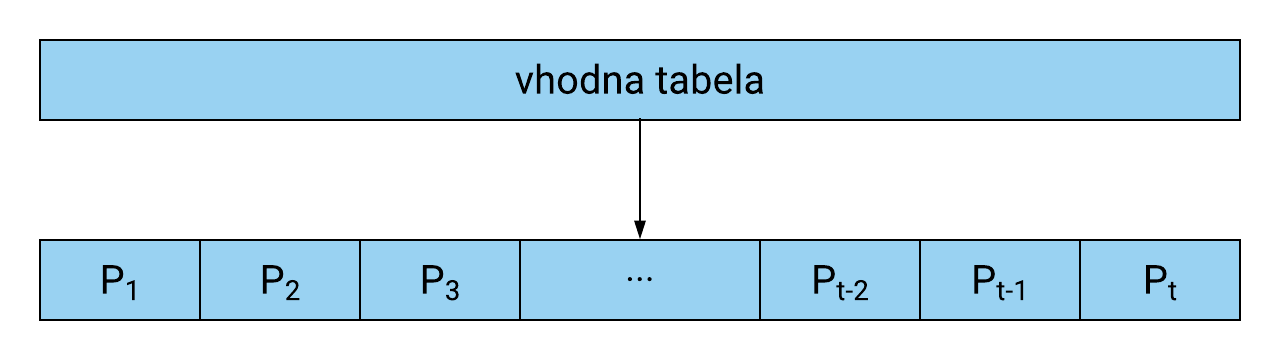
\includegraphics[width=0.45\textwidth]{aqs_diag_1}

Nato vsaka nit operira nad svojim delom tabele in uredi števila glede na pivot.
V L dobimo elemente manjše ali enake pivotu, v H pa elemente večje od pivota:

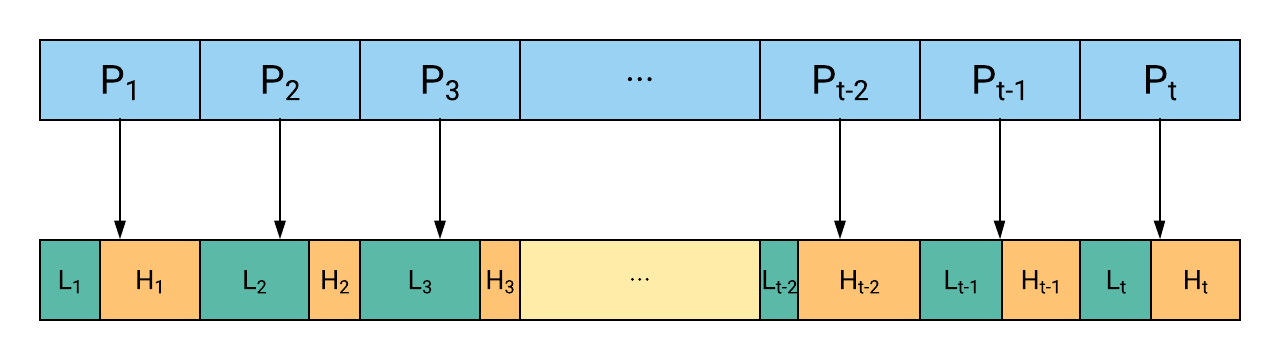
\includegraphics[width=0.45\textwidth]{aqs_diag_2}

Po urejanju vsaka nit sodeluje v premiku svojega dela elementov, ki so manjši ali enaki pivotu (L), na levo stran tabele.
Cilj koraka je, da niti združijo vse dele L in D tako, da ima tabela na levi vse L dele ter na desni vse D dele.
To pomeni, da bo pivot delil celotno tabelo na elemente, ki so manjši ali enaki pivotu in elemente, ki so večji od pivota. 
Zaradi pomnjenja odmika vsakega izmed delov lahko vsaka nit natačno izračuna, kam mora vsaka premakniti svoj del L. 

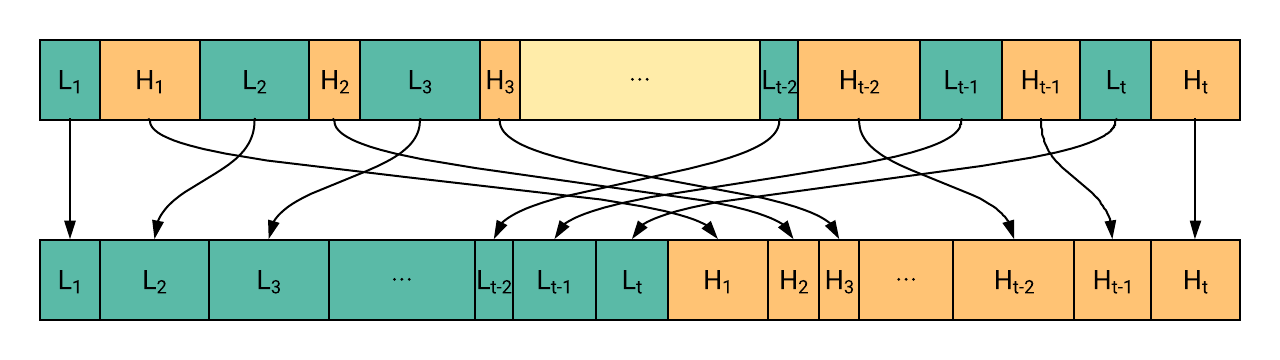
\includegraphics[width=0.45\textwidth]{aqs_diag_3}

Na koncu koraka se rekurzivno na obeh novo ustvarjenih delih tabele kliče naslednji korak v dveh ločenih nitih, vsaka dobi del nabora niti za delo:

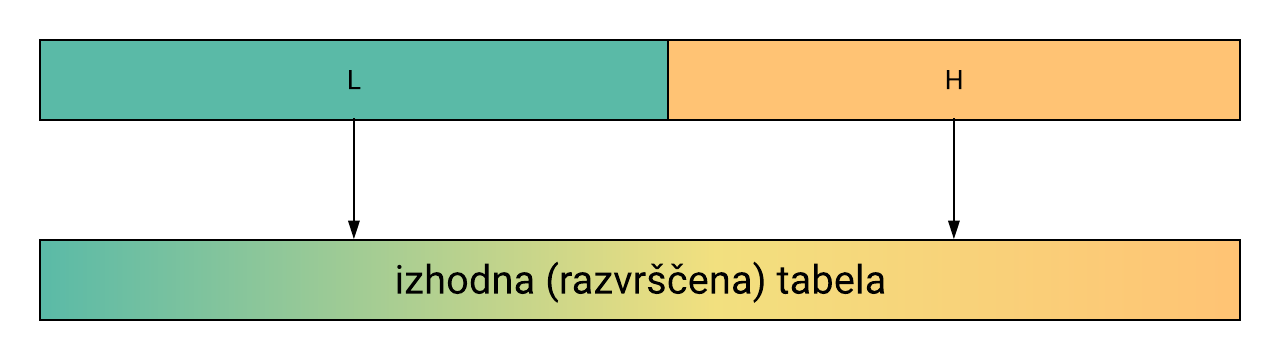
\includegraphics[width=0.45\textwidth]{aqs_diag_4}

Po koncu vseh rekurzivnih klicev je tabela sortirana.
Če je v nekem koraku na voljo le ena nit, se v tej niti izvede navaden Quick Sort.

Ta implementacija zahteva relativno veliko koordinacije med nitmi in usklajevanja velikosti delov.
Posledično zahteva več premisleka in dela kot le paralelizacija zanke.
Ta algoritem dobro pokaže prednosti in slabosti jezikov ko pride do fleksibilnosti paralelizacije.

\subsection{JPEG}

Format JPEG\footnote{https://en.wikipedia.org/wiki/JPEG} je eden izmed najbolj razširjenih digitalnih formatov za shranjevanje slik.
Za zmanjševanje količine podatkov, ki ga slike zasedajo, izrablja lastnosti človeškega vida - ljudje težje zaznamo spremembe pri visokofrekvenčnih
	komponentah slike kot pri nizkofrekvenčnih.

Kodiranje je sestavljeno iz treh glavnih delov, preslikave 8x8 kosov slike v frekvenčno domeno, kvantizacije in končnega stiskanja.

Preslikava je navadno diskretna kosinusna transformacija.\footnote{https://en.wikipedia.org/wiki/Discrete\_cosine\_transform}
Ta je implementirana kot množenje matrike vhodnih podatkov z matriko realnih koeficientov.

Kvantizacija poteka v treh korakih.
Najprej se podatki delijo z ustreznimi vrednostmi v kvantizacijski matriki.
Ta določa, katere frekvence naj se bolje ohranijo.
Nato se elementi matrike zaokrožijo na cela števila med -128 in 127.
Nazadnje pa se še matrika pretvori v vektor dolžine 64 prek poševnega cik-cak vzorca:

\begin{figure}[h]
\centering
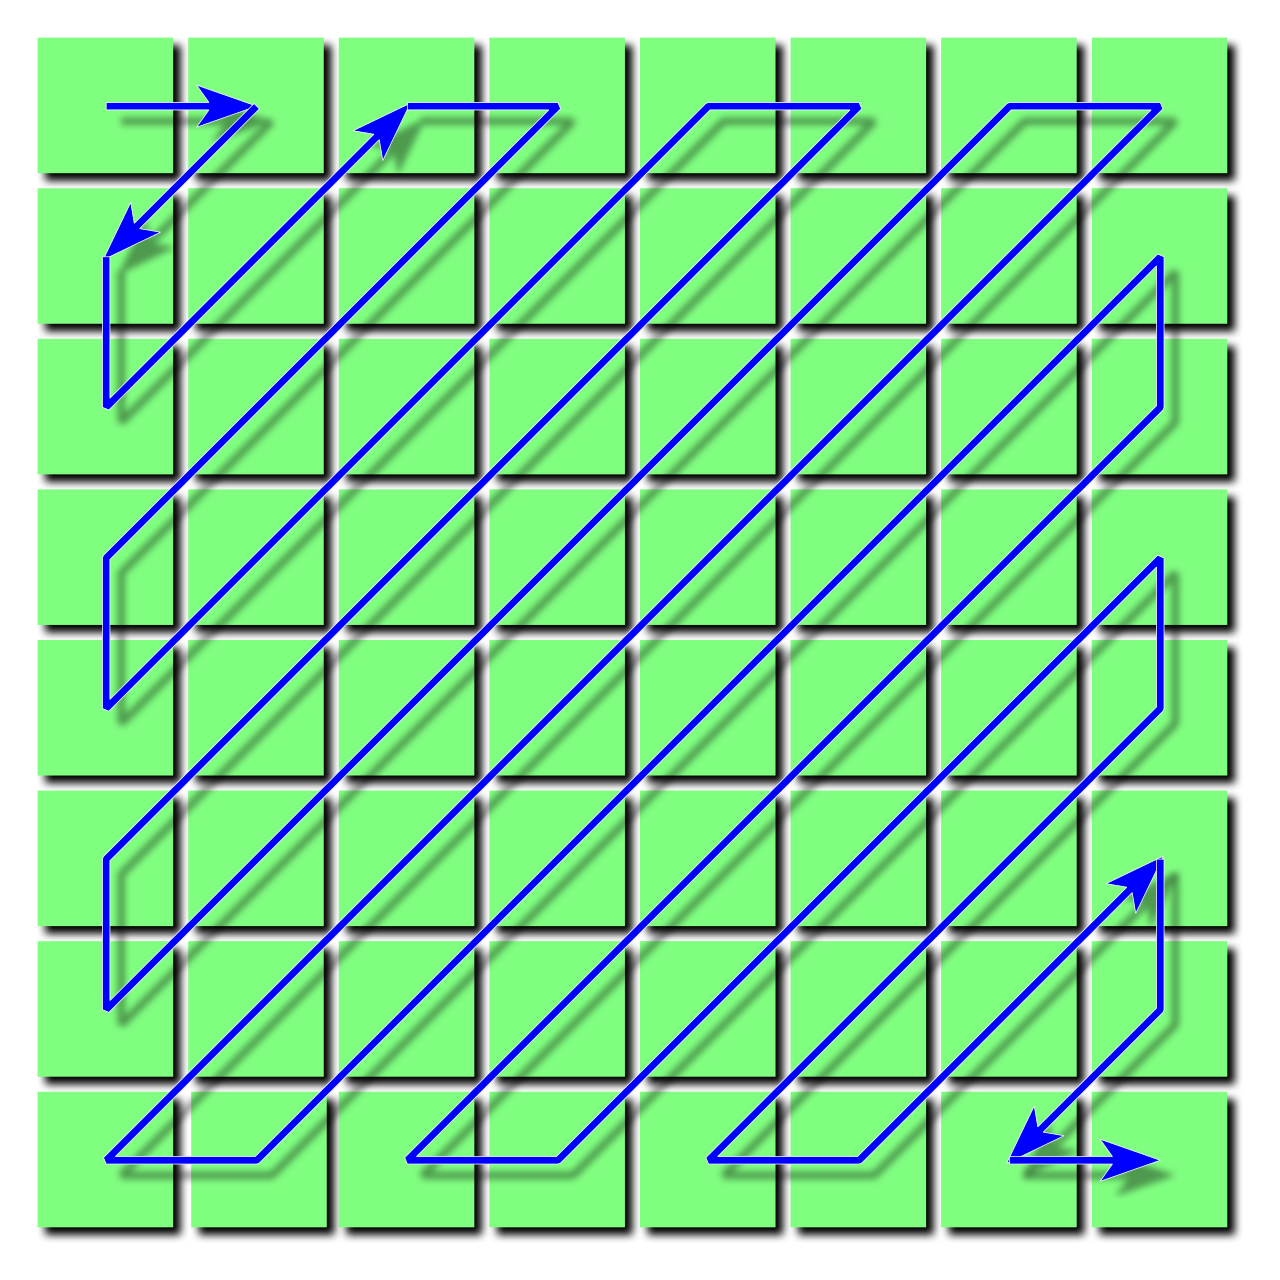
\includegraphics[width=0.35\textwidth]{jpeg_zigzag}
\caption{vir: Wikipedia}
\end{figure}

Končno stiskanje je brez izgub.
Navadno se uporablja Huffmanovo kodiranje.\footnote{https://en.wikipedia.org/wiki/Huffman\_coding}
Pri dobro izbrani kvantizacijski matriki se večina ničelnih elementov nahaja na koncu vektorja, kar lahko uporabimo, da podatke še bolj stisnemo.

Preslikava in prva dva koraka kvantizacije sta zelo primerna za izvajanje na GPE.
Algoritem simulira popačenje, ki se pojavi pri stiskanju, tako, da izvede DCT, deljenje s kvantizacijskimi vrednostmi in zaokroževanje, nato pa izvede
	obraten postopek, podatke množi s kvantizacijskimi vrednostmi in izvede inverzen DCT.

Ta algoritem je relativno enostaven pri implementaciji, je pa dovolj zahteven, da prikaže razlike med hitrostmi prevajanja in izvajanja programov na GPE
	med različnimi jeziki.

\section{Okolje}

Testirala sva na namiznem računalniku s procesorjem AMD Ryzen Threadripper 1920X na tovarniško nastavljeni hitrosti, 32 GB pomnilnika s hitrostjo
	3000 MHz in grafično kartico Nvidia GeForce GTX 1080 Ti.
Nameščen je bil operacijski sistem Windows 10 - 64 bit, različica 1809.

Programe v jeziku C/C++ sva prevajala in zaganjala v programskem okolju Microsoft Visual Studio 2017 z nastavitvami za “pthreads”, “OpenMP” in “OpenCL”
	kot je zapisano v navodilih za vaje pri predmetu Porazdeljeni sistemi.

Program v jeziku Python sva je zaganjala v ukaznem pozivu Powershell, Python verzija 3.7.1 64 bit, numpy verzija 1.15.4.

Programe v jeziku Julia sva zaganjala v ukaznem pozivu Powershell, Julia verzija 1.0.3 64 bit, CUDAnative verzija 0.9.1.

\section{Analiza hitrosti}

\subsection{Adaptive Quick Sort}

Algoritem očitno izpostavi obseg razlik hitrosti posameznih jezikov in kako velikost podatkov vpliva nanje.
Programe sva testirala na eksponento povečujoči tabeli naključno generiranih predznačenih 64-bitnih celih števil.
Za vsako velikost tabele sva vsak program izvedla petkrat in po koncu izvajanja izračunala povprečje izmerjenih časov sortiranj. 
Največja tabela je vsebovala 200 milijonov elementov.

Vsak program sva spisala na način, ki je minimiziral število nepotrebnih dostopov do pomnilnika in hkrati kar najbolje sledil prej opisanemu načrtu.
V primeru Pythona in Julie sva bila omejena s strani jezika, kar pa bo obravnavano kasneje.

\begin{figure}[h]
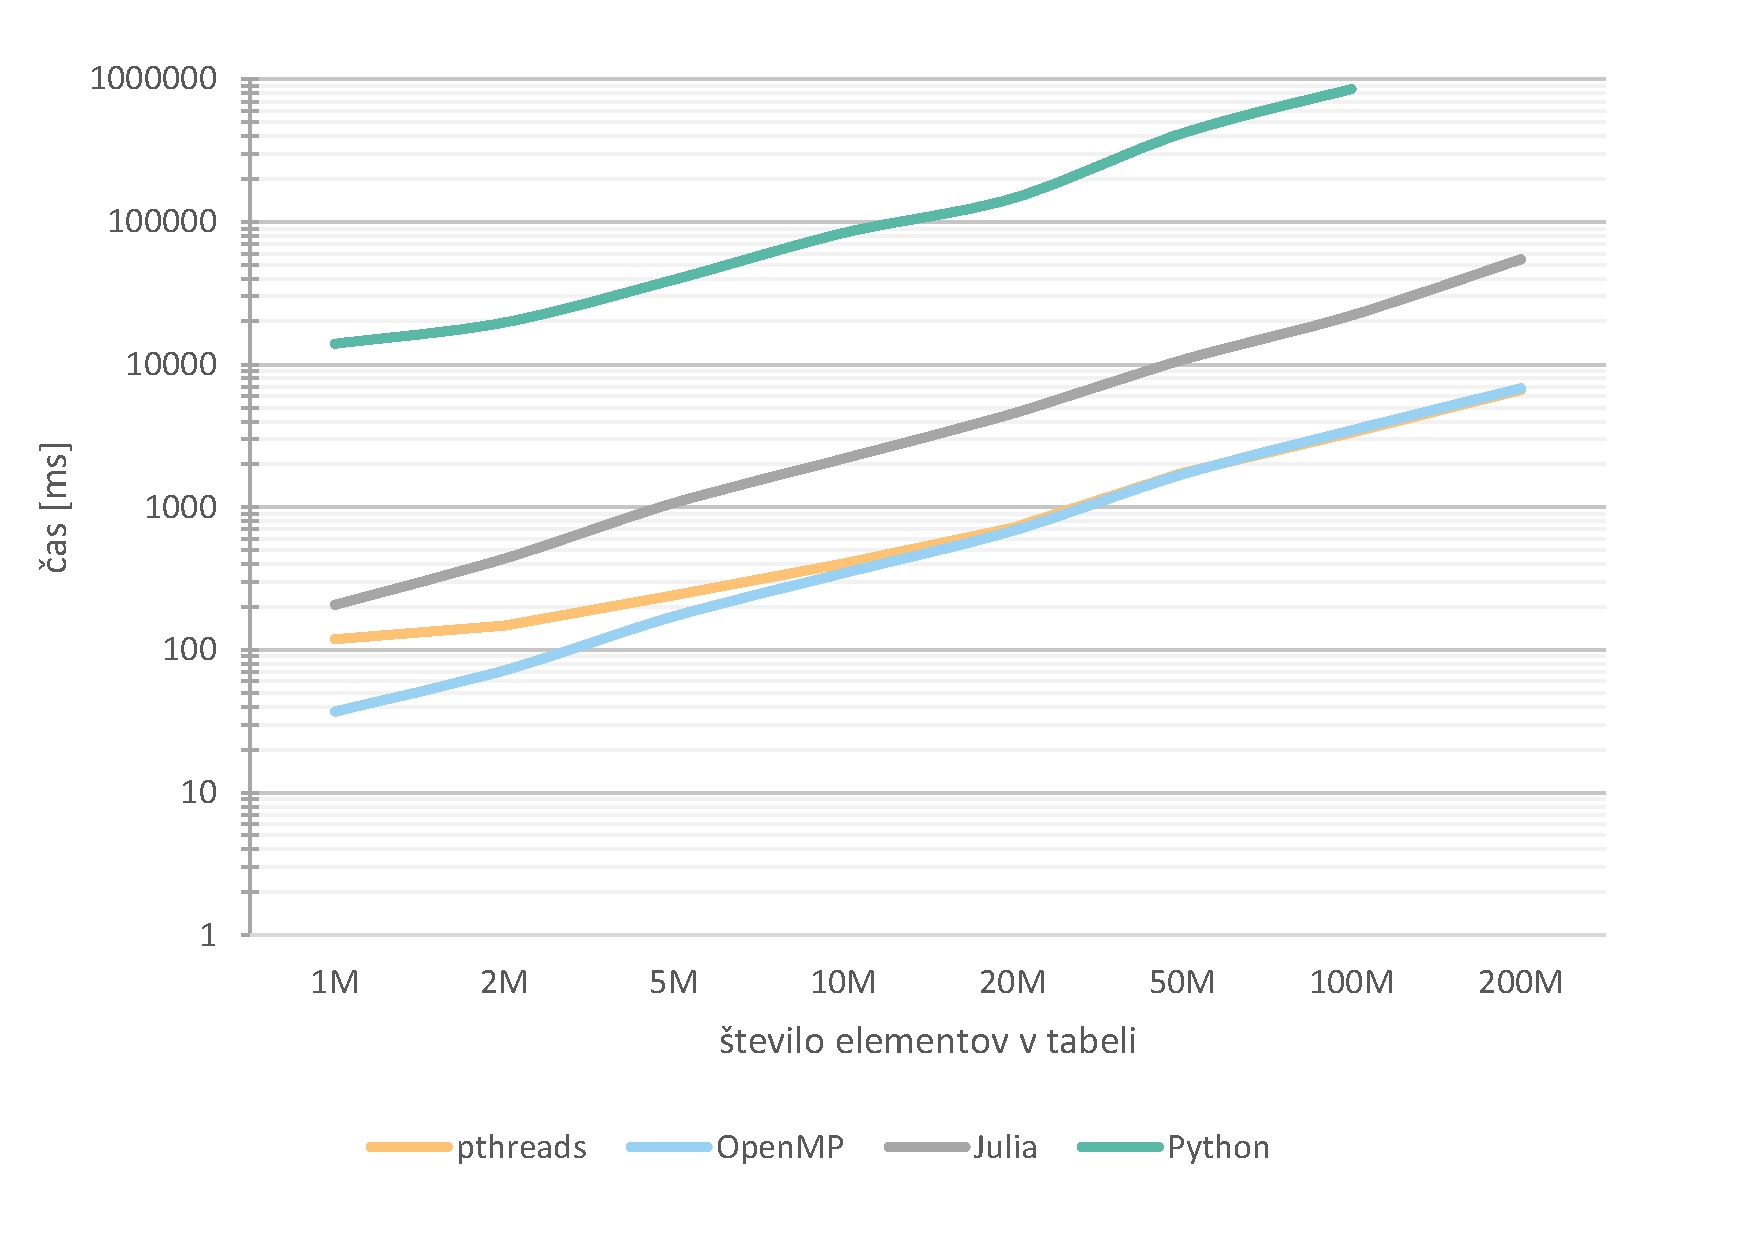
\includegraphics[width=0.5\textwidth]{aqs_speed}
\caption{Čas sortiranja tabele}
\end{figure}

Med pthreads in OpenMP je razlika največja pri majhnih tabelah, kjer je OpenMP veliko hitrejši.
Ta razlika se bolj ali manj izniči pri tabelah z več kot 20 milijoni elementov.

Julia je le slabo magnitudo počasnejša.
Za majhne tabele je skoraj tako hitra kot pthreads.
Med 2 in 20 milijoni elementov počasi izgublja hitrost.
Pri 200 milijonih pa nastopi težava s količino pomnilnika, zato se izvajanje še dodatno upočasni.

Python je od vseh jezikov najpočasnejši.
Pri 100 milijonih elementov doseže razmerje časa izvajanja v Pythonu s časom izvajanja s pthreads faktor 250.
Zaradi zelo dolgega časa testiranja pri tabeli velikosti 100 milijonov - približno 1 uro in 15 minut - se za 200 milijonov elementov ni testiralo.

\subsection{JPEG}

Za razliko od sortirnega algoritma sta tu implementaciji skoraj enakovredni.
Programa sva testirala na čedalje večjih kvadratnih slikah, velikosti dimenzij so bile naraščajoče potence števila 2.
Za vsako velikost sta se programa najprej dvakrat zagnala brez merjenja, kar odpravi počasen začetek izvajanja, nato pa je sledilo 5 meritev.
Končne vrednosti meritev sva povprečila.

Programa sta semantično skoraj identična.
Edine razlike so sintaktične, kjer se jezika razlikujeta.
Sicer pa je postopek izvajanja popolnoma enak, noben program ni optimiziran bolj kot drugi.

\begin{figure}[h]
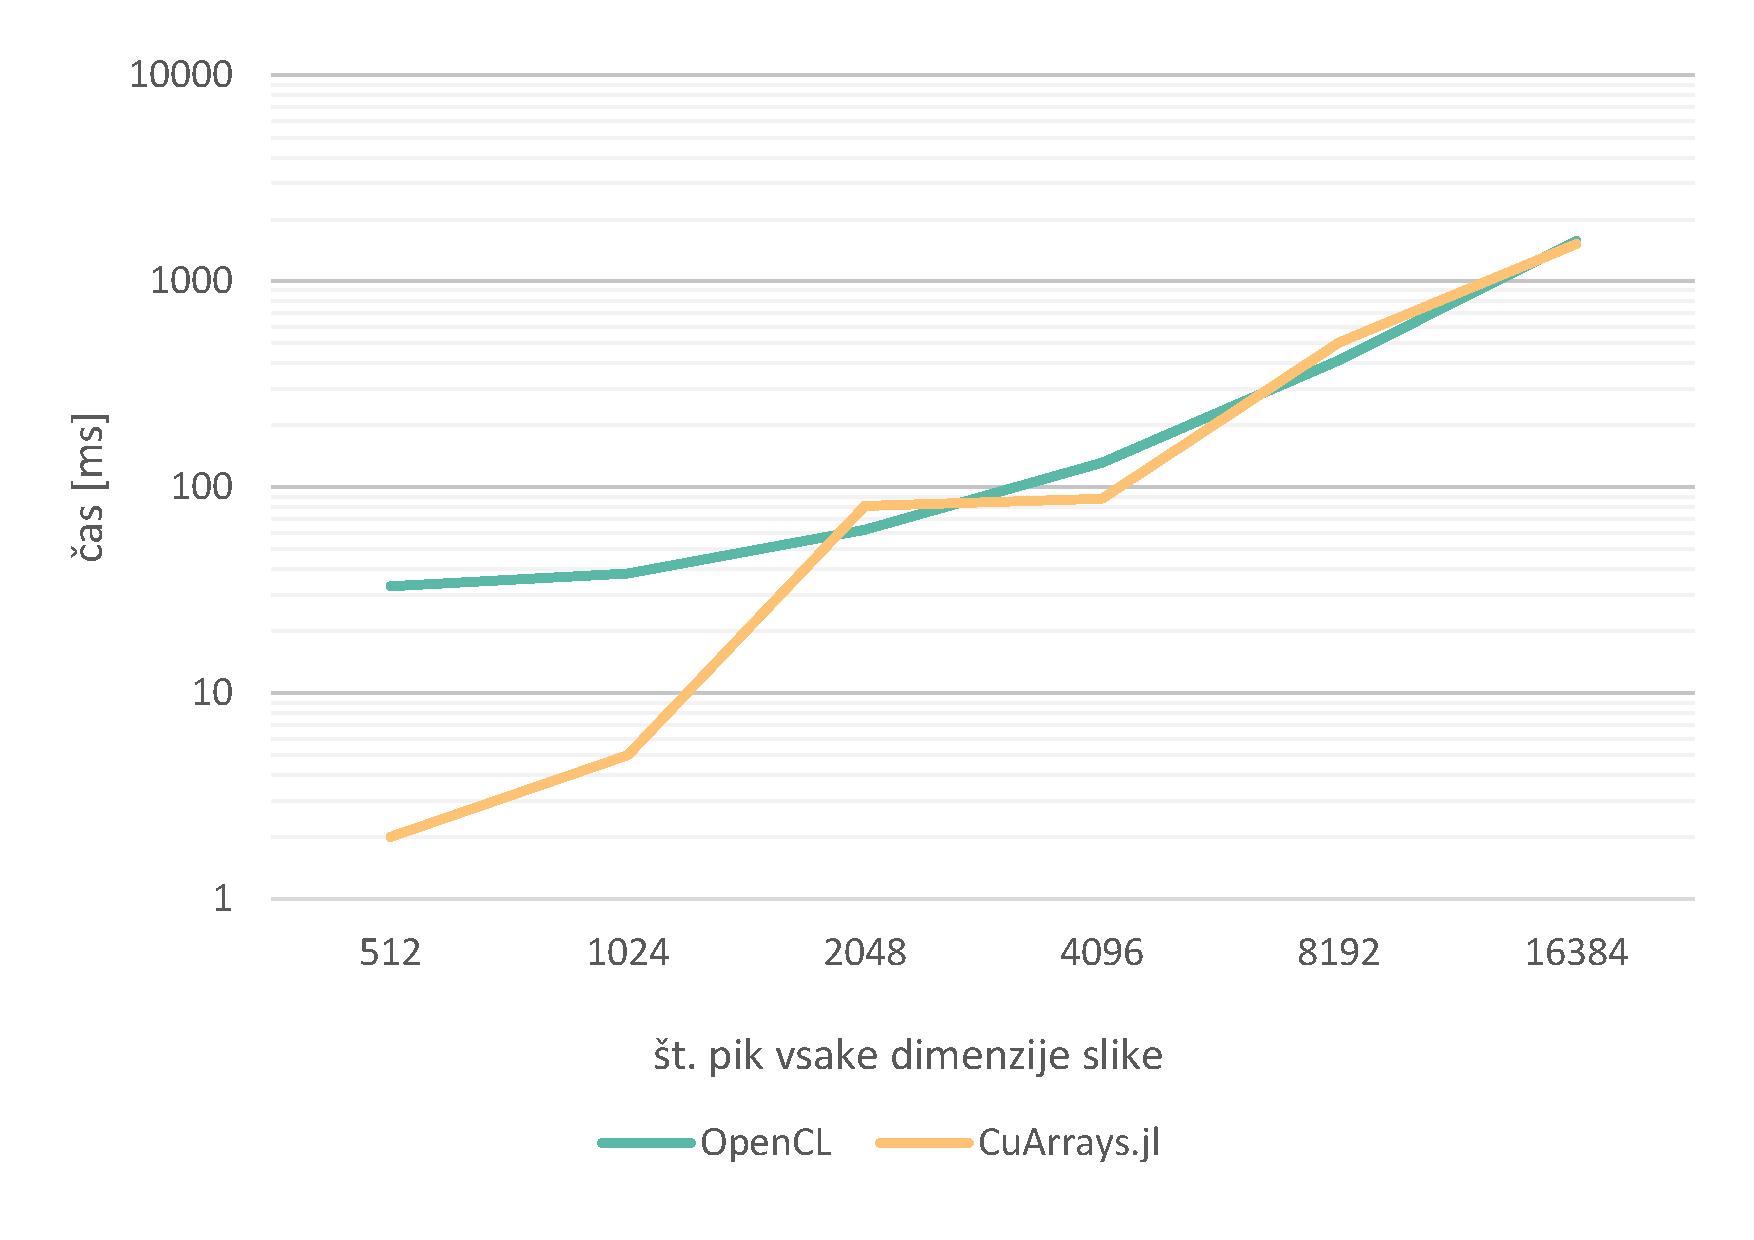
\includegraphics[width=0.45\textwidth]{jpeg_speed}
\caption{Čas simulacije JPEG popačenja brez prevajanja}
\end{figure}

Implemetacija CUDA vmesnika v jeziku Julia je v hitrosti za velike slike skoraj popolnoma primerljiva s C implementacijo vmesnika OpenCL.
Če zanemarimo čas prevajanja, je pri majhnih slikah Julia kar 15-krat hitrejša, ker med klici ohranja naložene funkcije v spominu GPE.

Zgodba se popolnoma obrne, če upoštevamo le prvi zagon skupaj s prevajanjem.
V okolju Visual studio od začetka prevajanja do konca shranjevanja preteče le slabih 5 sekund, ukazni poziv Julie pa porabi kar pol minute.

\section{Zahtevnost in izkušnja programiranja}

Hitrost izvajanja je le ena plat zgodbe.
Vse privarčevane sekunde ne pomenijo nič, če mora programer ure in ure razhroščevati težave brez ali s slabimi sporočili napak.

\subsection{C/C++}

C/C++ sta znana po svoji hitrosti in široki uporabnosti.

Večina jezikov deluje podobno in so bili modelirani prav po njiju.
Medtem ko C podpira uporabu struktur in predstavlja surovo osnovo je C++ objektno orientiran ter je njegova nadgradnja in razširitev. 

Izjemna podpora, kopica knjižnic in razširitev, služijo kot orodje za lažje delo.
Zaradi manjše abstrakcije v primerjavi z javo in pythonom je včasih programer prikrajšan na času in preprostosti kode.

V kolikor smo pripravljeni vložiti trud za kompleksnejšo rešitev problema lahko veliko pridobimo z optimizacijo in posledično dosežemo večje hitrosti pri
	izvajanju.

\subsection{Python}

Kodiranje je v Pythonu izjemno uporabniku prijazno.

Spremenljivke pridobijo tip na podlagi argumentov, ki jih prejmejo.
Če želimo spremeniti tip spremenljivke med izvajanjem, ji le priredimo novo vrednost.
Funkcije lahko definiramo med izvajanjem programa, prejmejo lahko argumente poljubnega tipa.

Če potrebujemo dodatno funkcionalnost, nam je na voljo vgrajen upravitelj paketov \texttt{pip}.
Ta nam omogoča prenos in namestitev več kot 160.000 zunanjih modulov, ki se pogosto posodabljajo.

Interpreter javi napako med izvajanjem in izpiše lokacijo v programu, kjer se je zgodila.
Zaradi dobre dokumentiranosti napak in ogromne skupnosti je iskanje rešitev enostavno.

Zaradi relativno visokega nivoja abstrakcije te prednosti pridejo na račun manjše hitrosti.
Poleg tega programerju ne omogoča zelo nizkonivojnega nadzora nad izvajanjem (vsaj CPython implementacija).
Zaradi tega in GIL je Python neprimeren kot jezik za visoko učinkovito računanje, vsaj v čisti obliki brez klicev v zunanje funkcije.

\subsection{Julia}

Julia predstavlja zanimivo sredino med C in Pythonom.
Zaradi prevajanja v zbirni jezik in optimizacije se v večini situacij po hitrosti približuje C-ju.
Hkrati pa so nam na voljo polni izpisi napak in dobra dokumentacija.
Jezik izpeljuje tipe, funkcije lahko defeniramo med izvajanjem, dopolnjujemo lahko vgrajene module, na voljo je vgrajen upravitelj paketov itd.

Največja hiba jezika trenutno je to, da ni še dokončan.
Veliko funkcionalnosti, ki so obljubljene kot del jezika, je še nedokončanih ali v eksperimentalnem stanju.

Primer nedokončane funkcionalnosti so niti.
Trenutno je makro \texttt{@threads} edini način za delitev dela med več niti.
V prihodnosti naj bi se spisal vmesnik, ki bo omogočal poljubno zaganjanje niti, ampak trenutno so implementirani le mutex-i, ki pa sami po sebi niso
	uporabni.

Poleg tega modul \texttt{OpenCL.jl} v času pisanja ni podpiral še Julie verzije 1.0.
Zaragi tega sva se odločila implementacijo JPEG simulacije spisati prek vmesnika CUDA.

\section{Sklep}

Julia je v konceptu zelo zanimiv jezik.
Prinaša obljubo hitrosti C-ja z enostavnostjo in prijaznostjo Pythona.
Večinoma se teh obljub tudi drži, kolikor je le možno.

Njena največja hiba je nedokončanost, kar pa ni presenetljivo, saj je šele lani dosegla izdajo 1.0.
Razvoj jezika je zelo hiter, tako zaradi fleksibilnosti jezika samega kot tudi vztrajno povečujoče se skupnosti.

Navdušenost nad jezikom Julia ni neupravičena.
Prinaša svež pristop do računanja, ki je modularen, prijazen in hiter.
Potrebuje le vztrajnost razvijalcev in čas.

\begin{thebibliography}{99}

% članek na spletni strani: \bibitem{tag} Avtor. (leto). Naslov. \emph{Stran/publikacija}. [Online] Dosegljivo: url. [Dostopano \today].
% študija: \bibitem{tag} Avtor, ``Naslov''. Institucija, (št.poročila, datum).

\bibitem{julia-site} The Julia Language. [Online] Dosegljivo: \mbox{https://www.julialang.org/}. [Dostopano \today].

\bibitem{julia-benchmarks} Julia Micro-Benchmarks. [Online] Dosegljivo: \mbox{https://www.julialang.org/benchmarks/}. [Dostopano \today].

\bibitem{julia-reasons} Why We Created Julia. [Online] Dosegljivo: \mbox{https://julialang.org/blog/2012/02/why-we-created-julia}. [Dostopano \today].

\bibitem{julia-metaprogramming} Metaprogramming. \emph{The Julia Language}. [Online] Dosegljivo:
	https://docs.julialang.org/\allowbreak en/v1/manual/\allowbreak metaprogramming/index.html. [Dostopano \today].
	
\bibitem{julia-multithreading} Multi-Threading (Experimental). \emph{The Julia Language}. [Online] Dosegljivo:
	https://docs.julialang.org/\allowbreak en/v1/\allowbreak manual/parallel-computing/\allowbreak index.html\allowbreak \#Multi-Threading-
	(Experimental). [Dostopano \today].

\bibitem{julia-thread-problems} hackguy. (2018). Threading issues. \emph{JuliaLang (discourse)}. [Online] Dosegljivo:
	https://discourse.julialang.org/t/threading-issues/18758. [Dostopano \today].

\bibitem{python-tiobe} TIOBE Index for January 2019. \emph{TIOBE Index}. [Online] Dosegljivo: https://www.tiobe.com/tiobe-index/. [Dostopano \today].

\bibitem{python-pypl} Pierre Carbonnelle (2018). PYPL PopularitY of Programming Language. [Online] Dosegljivo: http://pypl.github.io/PYPL.html.
	[Dostopano \today].

\bibitem{python-pypi} The Python Package Index. [Online] Dosegljivo: https://pypi.org/. [Dostopano \today].

\bibitem{python-gil} Global Interpreter Lock. \emph{Python Wiki}. [Online] Dosegljivo: https://wiki.python.org/moin/GlobalInterpreterLock.
	[Dostopano \today].

\end{thebibliography}

% that's all folks
\end{document}
